\documentclass{beamer}
\usetheme{metropolis}
\usepackage{graphicx}
\usepackage{tcolorbox}
\usepackage{subfig}
\title{Calculus-Based Physics-1: Mechanics (PHYS150-01): Unit 0}
\date{\today}
\author{Jordan Hanson}
\institute{Whittier College Department of Physics and Astronomy}

\begin{document}
\maketitle

\section{Opening Remarks - Welcome!}

\begin{frame}{Opening Remarks - Welcome!}
\small
\begin{figure}
\centering
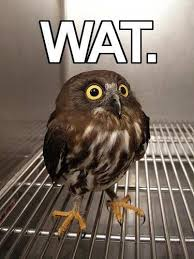
\includegraphics[width=0.27\textwidth]{../../watowl.jpeg}

\includegraphics[width=0.5\textwidth]{../../watTheDuck.png}
\caption{\label{fig:wat1} Taking physics for the first time.}
\end{figure}
\end{frame}

\section{Summary}

\begin{frame}{Week 1 Summary}
\textit{Physics} - $\phi\upsilon\sigma\iota\kappa\acute{\eta}$ - "phusik\'e": \textit{knowledge of nature} \\
from $\phi\acute{\upsilon}\sigma\iota\varsigma$ - "ph\'usis": \textit{nature}
\begin{enumerate}
\item Estimation/Unit Analysis - Chapters 1.1 - 1.4
\begin{itemize}
\item \alert{Estimating} the correct order of magnitude
\item \alert{Unit analysis} - dealing with the units of numbers
\end{itemize}
\item Coordinates and vectors - Chapters 2.1 - 2.4
\begin{itemize}
\item \alert{Scalars} and \alert{vectors}
\item \alert{Cartesian} (rectangular) coordinates, displacement
\item \alert{Vector} addition, subtraction, and multiplication
\end{itemize}
\item Review of Calculus Techniques
\begin{itemize}
\item The derivative, derivatives of elementary functions
\item \alert{Function} approximation
\item Anti-derivatives and integration
\end{itemize}
\end{enumerate}
\end{frame}

\section{Estimation/Unit Analysis - Chapters 1.1 - 1.4}

\begin{frame}{Estimation/Unit Analysis}
In science and engineering, \alert{estimation} is to obtain a quantity in the absence of precision, informed by rational constraints.
\begin{enumerate}
\item \textbf{Define relevant \alert{unit scales}}: (mg, g, or kg), (m/s or km/hr)
\item \textbf{Obtain \alert{complex quantities}} from simple ones
\begin{itemize}
\item Obtain \textit{areas} and \textit{volumes} from \textit{lengths}
\item Obtain \textit{rates} from \textit{numerators} and \textit{denominators}
\end{itemize}
\item \textbf{Taking advantage of \alert{scaling problems}}
\begin{itemize}
\item Knowing \textit{relationship} between variables
\item Using that \textit{relationship} to obtain new information
\end{itemize}
\item \textbf{Constrain the unknown with \alert{upper} and \alert{lower} limits}
\end{enumerate}
\end{frame}

\begin{frame}{Estimation/Unit Analysis}
\textbf{Units}: Which of the following represents a \textit{volume}?
\begin{itemize}
\item A: 10 gm
\item B: 10 cm$^2$
\item C: 1 cm$^3$
\item D: 1 cm s$^{-1}$
\end{itemize}
\end{frame}

\begin{frame}{Estimation/Unit Analysis}
\textbf{Units}: If a grain of sand within a fluid sinks 15 cm in 5 seconds, what is the speed of the grain?
\begin{itemize}
\item A: 3 cm
\item B: 3 s
\item C: 3 s/cm
\item D: 3 cm/s
\end{itemize}
\end{frame}

\begin{frame}{Estimation/Unit Analysis}
\textbf{Unit conversion}: If a person weights 120 lbs, what is their weight in kilograms?\footnote{One kilogram is 2.2 lbs.}
\begin{itemize}
\item A: 54.5 kg
\item B: 264 kg
\item C: 54.5 lbs
\item D: 264 lbs
\end{itemize}
\end{frame}

\begin{frame}{Estimation/Unit Analysis}
\textbf{Unit conversion}: A \alert{density} is a mass divided by a volume.  For example, water has a density of 1 gm cm$^{-3}$.  What is the density of water in kg m$^{-3}$?
\begin{itemize}
\item A: 1 kg m$^{-3}$
\item B: 10 kg m$^{-3}$
\item C: 100 kg m$^{-3}$
\item D: 1000 kg m$^{-3}$
\end{itemize}
\end{frame}

\begin{frame}{Estimation/Unit Analysis}
\textbf{Group exercise on complex units}: A \textit{vitrolero} is a classic container for serving \textit{agua fresca.}  It has a diameter of 20 cm, and a height of 30 cm.  How many cups can we serve from the vitrolero if we put 0.25 liters of agua fresca in each cup?
\begin{itemize}
\item \textit{Hint:} 1 liter is 1000 mL
\item \textit{Hint:} 1 mL is 1 cm$^3$
\item \textbf{Volume:} The volume of a cylinder is $\pi$ times the radius of the base, squared, times the height: $\pi r^2 h$.
\end{itemize}
\end{frame}

\begin{frame}{Estimation/Unit Analysis}
\textbf{Unit scale}: A generation is about one-third of a lifetime. Determine how many generations have passed since the year 0 AD\footnote{What is the appropriate scale here?}.
\begin{itemize}
\item A: $10$
\item B: $20$
\item C: $60$
\item D: $100$
\end{itemize}
\end{frame}

\begin{frame}{Estimation/Unit Analysis}
\textbf{Unit scale}: (a) What fraction of Earth’s diameter\footnote{The diameter of the Earth is 12,800 km.} is the greatest ocean depth (11 km below sea level)? (b) The greatest mountain height (8.8 km above sea level)?
\begin{itemize}
\item A: $8.6 \times 10^{-2}$, $6.9 \times 10^{-2}$
\item B: $8.6 \times 10^{-3}$, $6.9 \times 10^{-3}$
\item C: $8.6 \times 10^{-4}$, $6.9 \times 10^{-4}$
\item D: $8.6 \times 10^{-5}$, $6.9 \times 10^{-3}$
\end{itemize}
\end{frame}

\begin{frame}{Estimation/Unit Analysis}
\textbf{Complex quantities}: If a Whittier College athlete ran the 5k race at a track meet in 35 minutes, what was her average speed?
\begin{itemize}
\item A: 0.3 meters per second
\item B: 3 meters per second
\item C: 30 meters per second
\item D: 300 meters per second
\end{itemize}
\end{frame}

\begin{frame}{Estimation/Unit Analysis}
\textbf{Complex quantities}: Suppose you won the lottery and received \$1 billion USD.  Because your life is dope, you stack that paper over the Whittier College soccer field.  Each stack contains 100 bills, and each bill is worth \$100.  If you evenly cover the field, how high is the money level?
\begin{itemize}
\item A: 0.5 inch
\item B: 1 inch
\item C: 2 inches
\item D: 1 foot
\end{itemize}
\end{frame}

\begin{frame}{Estimation/Unit Analysis}
\textbf{Scaling problem}: Supposed you have an ideal gas in a cylinder of fixed volume.  If the pressure begins as 100 kPa, and you \textit{double} the temperature of the gas, what is the new pressure?
\begin{itemize}
\item A: 100 kPa
\item B: 50 kPa
\item C: 10 kPa
\item D: 200 kPa
\end{itemize}
\end{frame}

\begin{frame}{Estimation/Unit Analysis}
\textbf{Scaling problem}: Supposed you have an ideal gas in a cylinder of fixed volume.  If the pressure begins as 100 kPa, and you \textit{halve} the temperature of the gas, what is the new pressure?
\begin{itemize}
\item A: 100 kPa
\item B: 50 kPa
\item C: 10 kPa
\item D: 200 kPa
\end{itemize}
\end{frame}

\begin{frame}{Estimation/Unit Analysis}
\textbf{Upper/lower limits}: How many undergraduate students are there at Whittier College\footnote{What is the absolute lower limit, and what is the upper limit?}?
\begin{itemize}
\item A: 5,000
\item B: 1,000
\item C: 1,250
\item D: 500
\end{itemize}
\end{frame}

\begin{frame}{Estimation/Unit Analysis}
\textbf{Upper/lower limits}: What is the average yearly college tuition in the United States (before subtracting grants and scholarships)?
\begin{itemize}
\item A: \$5,000
\item B: \$10,000
\item C: \$25,000
\item D: \$40,000
\end{itemize}
What information affects the \alert{upper} and \alert{lower} limits here?
\end{frame}

\section{Coordinates and Vectors - Chapters 2.1 - 2.4}

\begin{frame}{Coordinates and Vectors - Applications: displacement}
\begin{tcolorbox}[colback=white,colframe=gray,title=Activity Link]
\textit{Who understands coordinates and vectors better than anyone else?} \\ \\
\url{https://youtu.be/0B7WL7nhIF4?si=_dl4t_GwL98aXWFa}
\end{tcolorbox}
\end{frame}

\begin{frame}{Coordinates and Vectors - Scalars, Vectors (Chapters 2.1-2.3)}
Physics requires \alert{mathematical objects} to build equations that capture the behavior of nature.  Two examples of such objects are \alert{scalar} and \alert{vector} quantities.  Each type of object obeys similar but different rules.
\begin{enumerate}
\item Scalar quantities
\begin{itemize}
\item mass: $m_1+(m_2+m_3) = (m_1+m_2)+m_3$
\item speed: $v_1(v_2+v_3) = v_1v_2+v_1v_3$
\item charge: $q_1 \left(\frac{1}{q_1}\right) = 1$, $q_1(0) = 0$
\end{itemize}
\item Vector quantities
\begin{itemize}
\item velocity: $\vec{v}_1 + (\vec{v}_2+\vec{v}_3) = (\vec{v}_1 + \vec{v}_2)+\vec{v}_3$
\item tension: $\vec{t}_1 \cdot (\vec{t}_2 + \vec{t}_3) = \vec{t}_1 \cdot \vec{t}_2 + \vec{t}_1 \cdot \vec{t}_3$
\end{itemize}
\end{enumerate}
\end{frame}

\begin{frame}{Coordinates and Vectors - Scalars, Vectors (Chapters 2.1-2.3)}
A vector may be expressed as \textit{a list of scalars}: $\vec{v} = (4,2)$ (a vector with two \textit{components}), $\vec{u} = (3,4,5)$ (three \textit{components}).  Now, we know how to add and subtract scalars.  How do we add and subtract vectors? \\
\vspace{0.5cm}
What is\\
$(1,3,8)+$\\ $(0,2,1)$? \\
Answer: $(1,5,9)$ \\
\vspace{0.5cm}
In other words, when adding vectors, we add them component by component.
\end{frame}

\begin{frame}{Coordinates and Vectors - Scalars, Vectors (Chapters 2.1-2.3)}
How do we subtract vectors? In the same fashion:\\
\vspace{0.5cm}
What is\\
$(1,3,8)-$\\ $(0,2,1)$? \\
Answer: $(1,1,7)$ \\
\vspace{0.5cm}
In other words, when subtracting vectors, we subtract them component by component.
\end{frame}

\begin{frame}{Coordinates and Vectors - Scalars, Vectors (Chapters 2.1-2.3)}
A HTML-based demonstration for adding vectors: \\
\vspace{0.5cm}
\url{https://phet.colorado.edu/en/simulations/vector-addition}
\vspace{0.5cm} \\
Notice several things:
\begin{itemize}
\item Produce vectors that \textit{cancel} each other.
\item What happens when vectors are parallel and orthogonal?
\end{itemize}
\end{frame}

\begin{frame}{Coordinates and Vectors - Scalars, Vectors (Chapters 2.1-2.3)}
How do we multiply vectors? In the same fashion, \textit{for one kind of multiplication}:\\
\vspace{0.5cm}
What is\\
$(1,3,8)\cdot (0,2,1)$? \\
Answer: $1\cdot 0 + 3 \cdot 2 + 8 \cdot 1 = 14$ \\
\vspace{0.5cm}
\textit{This kind of multiplication is known as the dot-product}.  There is also the \textit{cross-product}, which we will save for later.
\end{frame}

\begin{frame}{Coordinates and Vectors - Coordinates (Chapters 2.1-2.3)}
\small
The components of a vector may describe quantities in a \alert{coordinate system}, such as \textit{Cartesian coordinates} - after Ren\'e Descartes.  Vectors in the 3D Cartesian coordinate system (x,y,z) may be written in the following notation:
\\
\vspace{0.2cm}
$\boxed{\vec{v} = a\hat{i} + b\hat{j} + c\hat{k}}$
\\
\begin{itemize}
\item a: The amount in the +x-direction, $\hat{i}$: a vector of length 1, in the +x-direction
\item b: The amount in the +y-direction, $\hat{j}$: a vector of length 1, in the +y-direction
\item c: The amount in the +z-direction, $\hat{k}$: a vector of length 1, in the +z-direction
\end{itemize}
\end{frame}

\begin{frame}{Coordinates and Vectors - Vectors (Chapters 2.1-2.3)}
\begin{figure}
\centering
\subfloat[\label{fig:twovectors_a}]{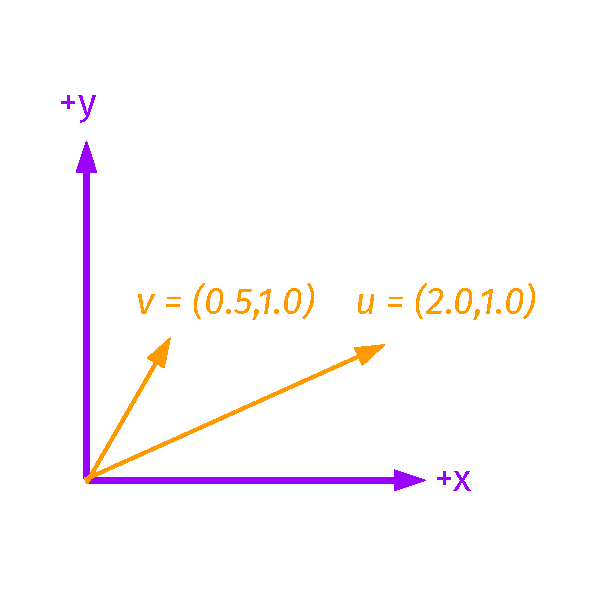
\includegraphics[width=0.45\textwidth,trim=1cm 1cm 1cm 1cm,clip=true]{figures/Vectors1.pdf}}
\subfloat[\label{fig:twovectors_b}]{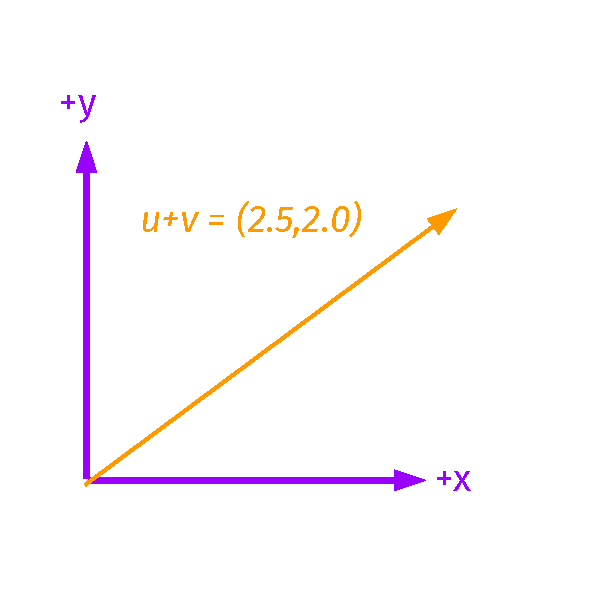
\includegraphics[width=0.45\textwidth,trim=1cm 1cm 1cm 1cm,clip=true]{figures/Vectors2.pdf}}
\caption{\label{fig:twovectors} (a) Two vectors in a two-dimensional Cartesian coordinate system: $\vec{u} = 0.5\hat{i}+1.0\hat{j}$ and $\vec{v} = 2.0\hat{i}+1.0\hat{j}$.  (b) What is $\vec{u}+\vec{v}$?  Adding components: $\vec{u}+\vec{v} = 2.5\hat{i}+2.0\hat{j}$.}
\end{figure}
\end{frame}

\begin{frame}{Coordinates and Vectors - Vectors (Chapters 2.1-2.3)}
\begin{figure}
\centering
\subfloat[\label{fig:twovectors_c}]{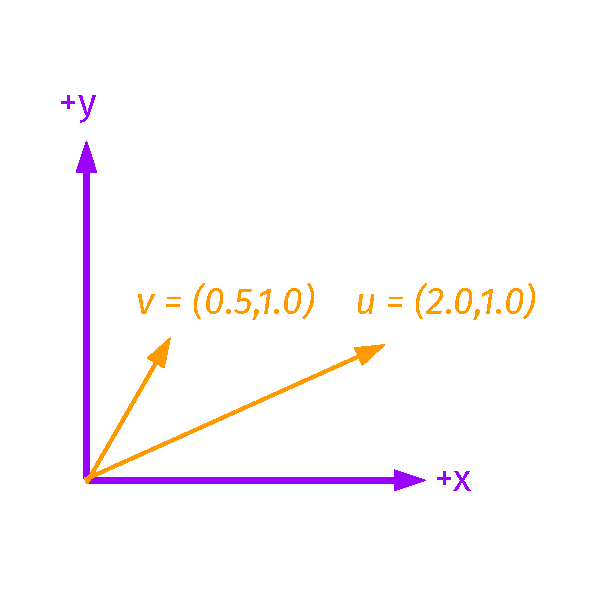
\includegraphics[width=0.45\textwidth,trim=1cm 1cm 1cm 1cm,clip=true]{figures/Vectors1.pdf}}
\subfloat[\label{fig:twovectors_d}]{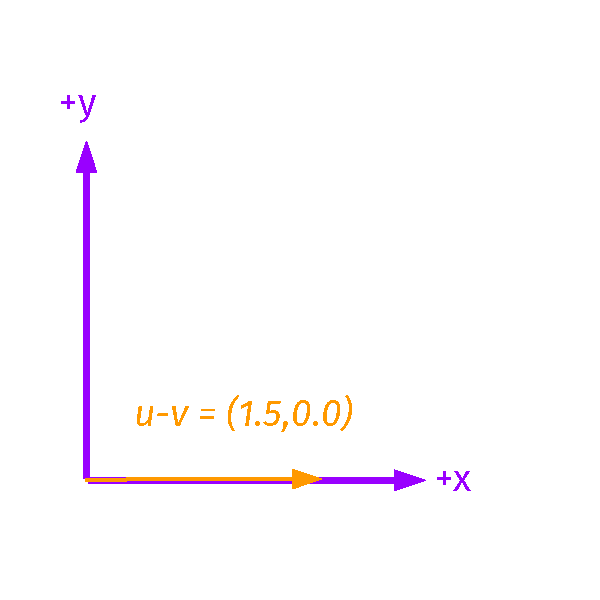
\includegraphics[width=0.45\textwidth,trim=1cm 1cm 1cm 1cm,clip=true]{figures/Vectors3.pdf}}
\caption{\label{fig:twovectors2} (a) Two vectors in a two-dimensional Cartesian coordinate system: $\vec{u} = 0.5\hat{i}+1.0\hat{j}$ and $\vec{v} = 2.0\hat{i}+1.0\hat{j}$.  (b) What is $\vec{u}-\vec{v}$?  Subtracting components: $\vec{u}-\vec{v} = 1.5\hat{i}+0.0\hat{j}$.}
\end{figure}
\end{frame}

\begin{frame}{Coordinates and Vectors - Vectors (Chapters 2.1-2.3)}
\begin{figure}
\centering
\subfloat[\label{fig:twovectors_e}]{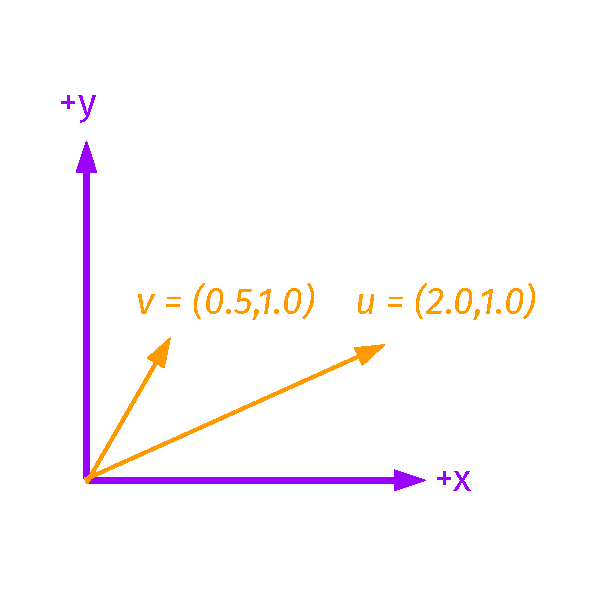
\includegraphics[width=0.45\textwidth,trim=1cm 1cm 1cm 1cm,clip=true]{figures/Vectors1.pdf}}
\subfloat[\label{fig:twovectors_f}]{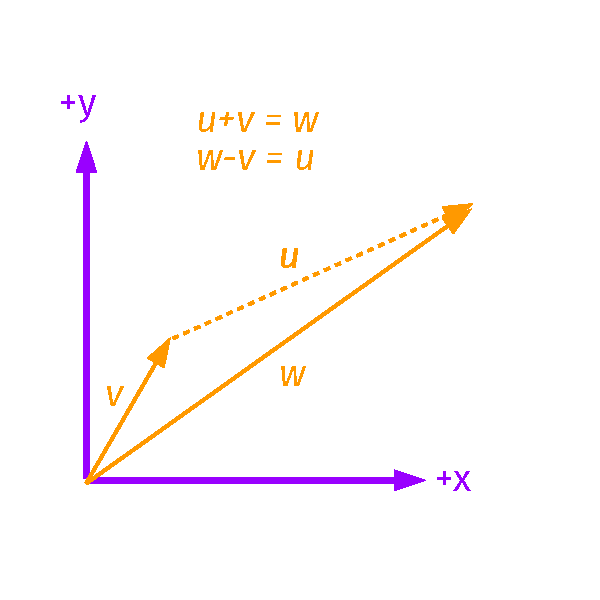
\includegraphics[width=0.45\textwidth,trim=1cm 1cm 1cm 1cm,clip=true]{figures/Vectors4.pdf}}
\caption{\label{fig:twovectors3} (a) Two vectors in a two-dimensional Cartesian coordinate system: $\vec{u} = 0.5\hat{i}+1.0\hat{j}$ and $\vec{v} = 2.0\hat{i}+1.0\hat{j}$.  (b) To compute $\vec{w}-\vec{v}$, arrange the vectors to get a sense of the result, $\vec{u}$.}
\end{figure}
\end{frame}

\begin{frame}{Coordinates and Vectors - Vectors (Chapters 2.1-2.3)}
\small
\begin{minipage}[b]{0.45\linewidth}
$\vec{p} = 4\hat{i}+2\hat{j}$.  $\vec{q} = -4\hat{i}+2\hat{j}$.  \\
Compute $\vec{p} \cdot \vec{q}$.
\vspace{0.2cm}
\begin{itemize}
\item A: 12
\item B: -12
\item C: 4
\item D: 8
\end{itemize}
\end{minipage}
\hspace{0.5cm}
\begin{minipage}[b]{0.45\linewidth}
$\vec{p} = -1\hat{i}+6\hat{j}$.  $\vec{q} = 3\hat{i}+0.5\hat{j}$.  \\
Compute $\vec{p} \cdot \vec{q}$.
\vspace{0.2cm}
\begin{itemize}
\item A: -1
\item B: 1
\item C: 0
\item D: 3
\end{itemize}
\end{minipage}
\end{frame}

\begin{frame}{Coordinates and Vectors - Vectors (Chapters 2.1-2.3)}
Why was the last answer zero?  Look at it graphically:
\begin{figure}
\centering
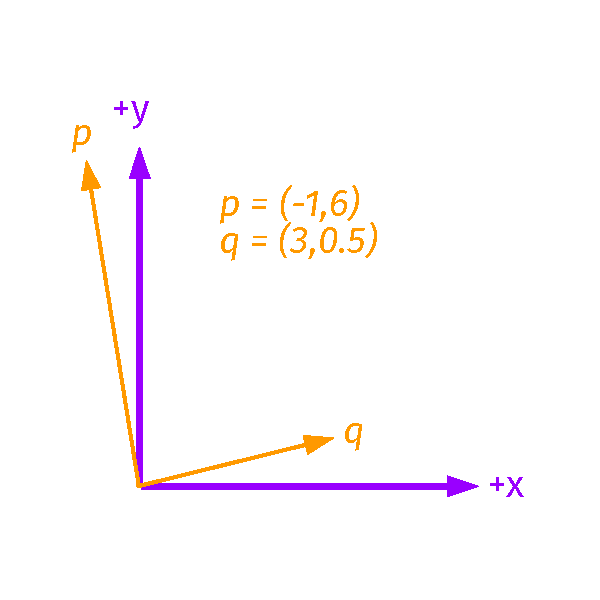
\includegraphics[width=0.5\textwidth,trim=1cm 1cm 1cm 1cm,clip=true]{figures/Vectors5.pdf}
\caption{\label{fig:twovectors4} Two vectors $\vec{p}$ and $\vec{q}$ are \textit{orthogonal} if $\vec{p} \cdot \vec{q} = 0$.}
\end{figure}
\end{frame}

\begin{frame}{Coordinates and Vectors - Vectors (Chapters 2.1-2.3)}
What if the vectors are parallel? Look at it graphically:
\begin{figure}
\centering
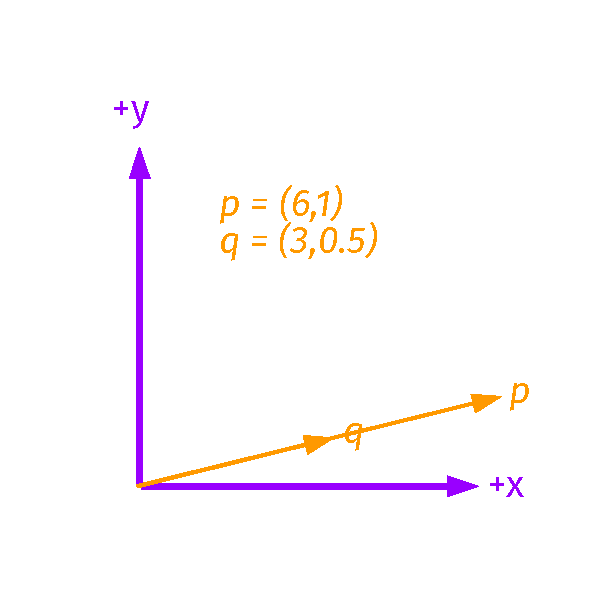
\includegraphics[width=0.5\textwidth,trim=1cm 1cm 1cm 1cm,clip=true]{figures/Vectors6.pdf}
\caption{\label{fig:twovectors5} Two vectors $\vec{p}$ and $\vec{q}$ are \textit{parallel} if $\vec{p} \cdot \vec{q}$ is maximal.}
\end{figure}
\end{frame}

\begin{frame}{Coordinates and Vectors - Dot Product (Chapters 2.1-2.3)}
The \textit{length} or \textit{norm} of a vector $\vec{v} = a\hat{i}+b\hat{j}$ is $|\vec{v}| = \sqrt{a^2+b^2}$.\\
\begin{figure}
\centering
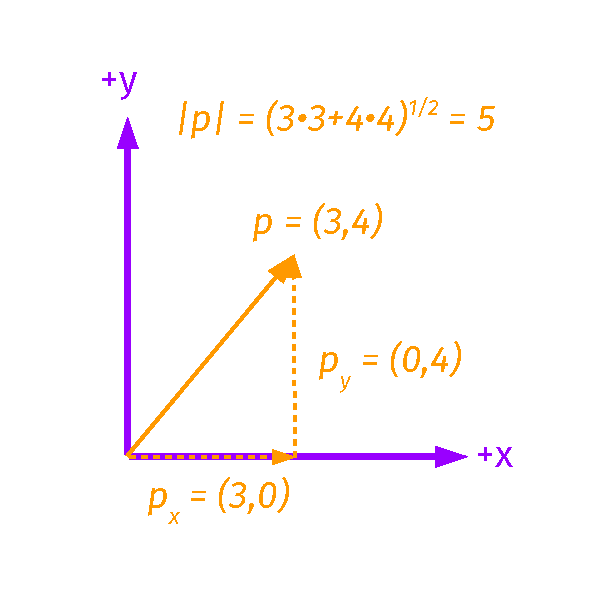
\includegraphics[width=0.5\textwidth,trim=1cm 1cm 1cm 1cm,clip=true]{figures/Vectors7.pdf}
\caption{\label{fig:twovectors6} Computing the norm of a vector $\vec{p}$.}
\end{figure}
\end{frame}

\begin{frame}{Coordinates and Vectors - Dot Product (Chapters 2.1-2.3)}
Notice that $\sqrt{\vec{p}\cdot\vec{p}} = |\vec{p}|$.\\
Let $\theta_p$ be the angle between $\vec{p}$ and the x-axis.  \\
$p_{x} = \vec{p} \cdot \hat{i} = |\vec{p}| \cos(\theta_{p})$. \\
$p_{y} = \vec{p} \cdot \hat{j} = |\vec{p}| \sin(\theta_{p})$.\\
\vspace{0.5cm}
\textit{Theorem:} The dot product of two vectors $\vec{p}$ and $\vec{q}$ is $|u||v|\cos(\theta)$, if $\theta$ is the angle between them.\\
\vspace{0.5cm}
\textit{Proof}: $\vec{p}\cdot\vec{q} = p_{x}q_{x} + p_{y}q_{y} = |p||q|\cos\theta_p\cos\theta_q+|p||q|\sin\theta_q\sin\theta_q$ \\
$=|p||q|(\cos\theta_p\cos\theta_q+\sin\theta_p\sin\theta_q) = |p||q|\cos(\theta_p-\theta_q)$ \\
$=|p||q|\cos\theta$. \\
\vspace{0.1cm}
$\boxed{\vec{p}\cdot\vec{q}=|p||q|\cos\theta}$
\end{frame}

\begin{frame}{Coordinates and Vectors - Dot Product (Chapters 2.1-2.3)}
\small
\begin{minipage}[b]{0.45\linewidth}
An object moves at 2 m/s at $\theta = 60^{\circ}$ with respect to the x-axis.  What is the velocity of the object?
\vspace{0.2cm}
\begin{itemize}
\item A: $(1\hat{i}$ + $1\hat{j})$  m/s
\item B: $(\sqrt{3}\hat{i}$ + $1\hat{j})$  m/s
\item C: $(\sqrt{3}\hat{i}$ + $\sqrt{3}\hat{j})$  m/s
\item D: $(1\hat{i}$ + $\sqrt{3}\hat{j})$  m/s
\end{itemize}
\end{minipage}
\hspace{0.5cm}
\begin{minipage}[b]{0.45\linewidth}
What is the dot product of this velocity with another velocity: 5 m/s along the x-axis?
\vspace{0.7cm}
\begin{itemize}
\item A: 1 (m/s)$^2$
\item B: 5 (m/s)$^2$
\item C: 10 (m/s)$^2$
\item D: 5 (m/s)
\end{itemize}
\end{minipage}
\end{frame}

\begin{frame}{Coordinates and Vectors - Scalars, Vectors (Chapters 2.1-2.3)}
Is it possible to multiply vectors and scalars?  Of course: $a_1\vec{p} = a_1p_x\hat{i}+a_1p_y\hat{j}$.\\
\vspace{0.2cm}
Also, multiplication properties still hold.  For example: $(a_1+a_2)\vec{p} = a_1\vec{p}+a_2\vec{p}$. \\
\vspace{0.2cm}
\small
A spacecraft moves at 400 m/s, at an angle of 30 degrees with respect to the x-axis.  If it fires two thrusters that boost the x-component and y-component of the velocity by 25\% and 50\%, respectively, what is the final velocity?
\begin{itemize}
\item A: $(433\hat{i}+300\hat{j})$ m/s
\item B: $(300\hat{i}+433\hat{j})$ m/s
\item C: 400 m/s
\item D: $(400\hat{i}+433\hat{j})$ m/s
\end{itemize}
\end{frame}

\begin{frame}{Coordinates and Vectors - Dislacement (Chapters 2.1-2.3)}
We define the \textit{position} of an object as a vector locating it in a given coordinate system.  The scalar \textit{distance} is the norm of the position vector, that is, the distance to to the origin. \\
\vspace{0.5cm}
Now we can introduce the concept of \alert{dislacement}: a vector describing a movement of an object.
\end{frame}

\begin{frame}{Coordinates and Vectors - Displacement (Chapters 2.1-2.3)}
\begin{figure}
\centering
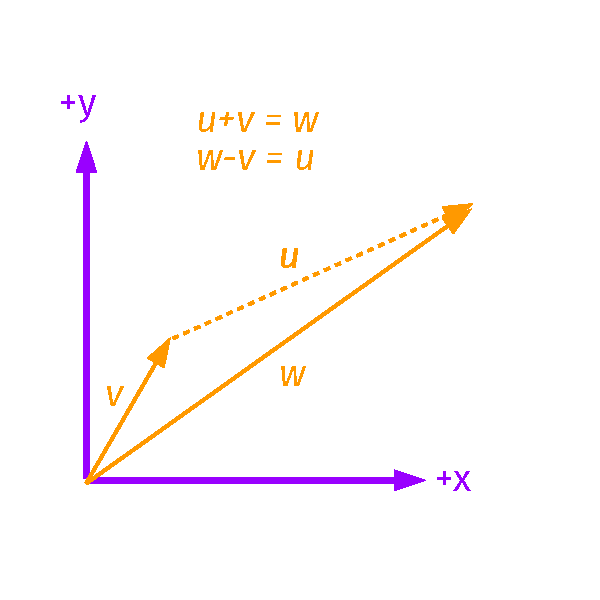
\includegraphics[width=0.52\textwidth]{figures/Vectors4.pdf}
\caption{\label{fig:displacement} Suppose an object moves from position $\vec{v}$ to $\vec{w}$.  In this case, the \alert{displacement} is $\vec{u}$. \textbf{Thus, the final position is the initial position, plus the displacement.}}
\end{figure}
\end{frame}

\begin{frame}{Coordinates and Vectors - Displacement (Chapters 2.1-2.3)}
It follows that the \textit{displacement} is zero if the initial and final positions are the same, but the \textit{distance travelled} is not.\\
\vspace{0.2cm}
\small
Suppose a jet fighter travelling at 800 km per hour banks such that it flies in a circle of radius 0.5 km.  How long does it take to complete the circle?  What is the distance traveled, and what is the displacement?
\begin{itemize}
\item A: $2\pi$ km, 28 seconds, $2\pi$ km
\item B: $\pi$ km, 14 seconds, $\pi$ km
\item C: $\pi$ km, 28 seconds, $\pi$ km
\item D: $\pi$ km, 14 seconds, $0$ km
\end{itemize}
\end{frame}

\begin{frame}{Coordinates and Vectors - Average Velocity  (Chapter 3.1)}
\alert{Average velocity} is the ratio of the \alert{displacement} to the elapsed time.\\
\begin{equation}
\boxed{\vec{v}_{\rm avg} = \frac{\Delta \vec{x}}{\Delta t}}
\end{equation}
The \textit{average speed} is the norm of the average velocity:
\begin{equation}
\boxed{v_{\rm avg} = \frac{|\Delta \vec{x}|}{\Delta t}}
\end{equation}
If the motion is in one dimension, then the average speed is
\begin{equation}
v_{\rm avg} = \frac{x_{\rm f} - x_{\rm i}}{t_{\rm f} - t_{\rm i}}
\end{equation}
\end{frame}

\begin{frame}{Coordinates and Vectors - Average Velocity (Chapter 3.1)}
\begin{figure}
\centering
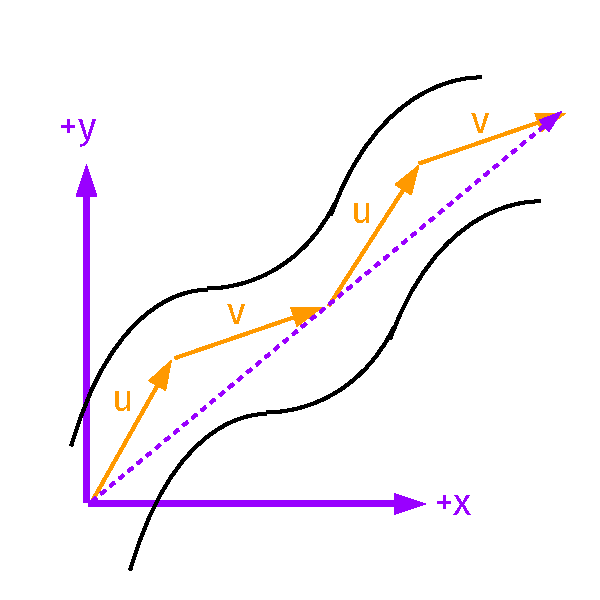
\includegraphics[width=0.52\textwidth]{figures/AveVelocity.pdf}
\caption{\label{fig:avevel} A Formula-1 driver keeps his car on the track by following a path approximated by the position vectors $u$, $v$, $u$, and $v$.  The dashed arrow represents the total displacement.}
\end{figure}
\end{frame}

\begin{frame}{Coordinates and Vectors - Average Velocity (Chapter 3.1)}
If $\vec{u} = (20\hat{i}+30\hat{j})$ m, and $\vec{v} = (30\hat{i}+20\hat{j})$ m, what is the total displacement?  If the elapsed time is 10 seconds, what is the average velocity? \\
\vspace{0.2cm}
\begin{itemize}
\item A: $(50\hat{i} + 50\hat{j})$ m, 14 m/s
\item B: $(80\hat{i} + 100\hat{j})$ m, 10 m/s
\item C: $(100\hat{i} + 100\hat{j})$ m, 14 m/s
\item D: $(50\hat{i} + 150\hat{j})$ m, 10 m/s
\end{itemize}
\end{frame}

\section{Review of Calculus Techniques}

\begin{frame}{Review of Calculus Techniques}
\begin{enumerate}
\item \textbf{Computing limits}
\begin{itemize}
\item Examples in mathematics
\item Examples in physics
\end{itemize}
\item \textbf{Differentiation}
\begin{itemize}
\item Definition of the derivative
\item Examples of derivatives
\end{itemize}
\item \textbf{Integration}
\begin{itemize}
\item Definition of the integral
\item Examples of integrals
\end{itemize}
\end{enumerate}
\end{frame}

\begin{frame}{Review of Calculus Techniques - Computing Limits}
\small
Consider the function $f(x)$, defined below:
\begin{equation}
f(x) = \frac{1}{1+x^2}
\end{equation}
\textbf{Evaluate} the function at the following points:
\begin{itemize}
\item $x = 0$
\item $x = 10$
\item $x = 100$
\item $x = 1000$
\end{itemize}
What is the \textit{limiting value} of the function as $x \to \infty$?  What is the \textit{limiting value} of the function as $x \to -\infty$?
\end{frame}

\begin{frame}{Review of Calculus Techniques - Computing Limits}
\small
Consider the function $f(x)$, defined below:
\begin{equation}
f(x) = \exp(x) = e^x
\end{equation}
\textbf{Evaluate} the function at the following points:
\begin{itemize}
\item $x = 0$
\item $x = 10$
\item $x = 100$
\item $x = 1000$
\end{itemize}
What is the \textit{limiting value} of the function as $x \to \infty$?  What is the \textit{limiting value} of the function as $x \to -\infty$?
\end{frame}

\begin{frame}{Review of Calculus Techniques - Computing Limits}
\small
Consider the function $f(x)$, defined below:
\begin{equation}
f(x) = \sin(x)
\end{equation}
\textbf{Evaluate} the function at the following points:
\begin{itemize}
\item $x = \pi$
\item $x = -\pi$
\item $x = 0.1$
\item $x = 0.01$
\end{itemize}
What is the \textit{limiting value} of the function as $x \to 0$?  The procedure is straightforward if the function is \textit{continuous} and \textit{differentiable}.
\end{frame}

\begin{frame}{Review of Calculus Techniques - Differentiation}
\small
\begin{tcolorbox}[colback=white,colframe=gray,title=Derivative of a Function]
Let $f(t)$ be a continuous function on an interval $[a,b]$, and $a<t<b$.  The derivative of $f(t)$ is
\begin{equation}
f'(t) = \frac{df}{dt} = lim_{\Delta t \to 0} ~ \frac{f(t+\Delta t) - f(t)}{\Delta t}
\end{equation}
\end{tcolorbox}
\begin{tcolorbox}[colback=white,colframe=gray,title=List of Common Derivatives]
Here is a link to lists of common derivatives:
\url{https://en.wikipedia.org/wiki/Derivative} \\
\url{https://en.wikipedia.org/wiki/Differentiation_rules}
\end{tcolorbox}
\textbf{Professor:} work some examples.
\end{frame}

\begin{frame}{Review of Calculus Techniques - Integration}
\begin{tcolorbox}[colback=white,colframe=gray,title=Integral of a Function]
Let $f(t)$ be a continuous function on an interval $[a,b]$, and $a<t_i<b$, where $t_i$ are regular points within the integral.  The Riemann integral is
\begin{equation}
I = \sum_i f(t_i) \Delta t_i \to \int_a^b f(t) dt
\end{equation}
\end{tcolorbox}
\begin{tcolorbox}[colback=white,colframe=gray,title=List of Common Derivatives]
Here is a link to a list of common integrals:
\url{https://en.wikipedia.org/wiki/Lists_of_integrals}
\end{tcolorbox}
\textbf{Professor:} work some examples.
\end{frame}

\section{Conclusion}

\begin{frame}{Week 1 Summary}
\begin{enumerate}
\item Methods of approximation
\begin{itemize}
\item \alert{Estimating} the correct order of magnitude
\item \alert{Function} approximation
\item \alert{Unit analysis}
\end{itemize}
\item Coordinates and vectors
\begin{itemize}
\item \alert{Scalars} and \alert{vectors}
\item \alert{Cartesian} (rectangular) coordinates, displacement
\item \alert{Vector} addition, subtraction, and multiplication
\end{itemize}
\item Review of Calculus Techniques
\begin{itemize}
\item Limits
\item Differentiation
\item Integration
\end{itemize}
\end{enumerate}
\end{frame}

\end{document}
